
\documentclass{article}
\usepackage[left=1cm,right=1cm]{geometry}
\usepackage{float}

\usepackage[htt]{hyphenat}
\usepackage{graphicx}
\usepackage{courier}
\usepackage{siunitx}


\begin{document}

\title{Fast oven controller guide}
\date{\today}

\maketitle


\section{Safety interlocks}
There are several layers of interlock that should protect us from unintentionally
demolishing our ovens.

The first layer of interlock sets an error flag and disables the PWM module if a
fault condition is detected. If the PWM module is disabled, the PIC pin reverts
to an input. The H-bridge driver detects this (pull to mid-rail) and shuts down,
safeing the system. The conditions that trigger this interlock are:
\begin{itemize}
\item \textbf{Temperature:}
If any temperature reading is outside the valid range. This protects
against thermocouple faults (open, short, inverted), temperature typos (!), and
oscillating PI controllers.
\item \textbf{Current:}
If any current readying is above the limit. This protects against
oscillating PI controllers or gross temperature errors.
\item \textbf{Burn time:}
If the duty-cycle has been non-zero for longer than the limit. This stops the
oven burning forever if there are communication bugs, the Beaglebone crashes, or
the controlling experiment crashes.
\item \textbf{ADC CRC:}
If several ADC data CRCs fail in a given time window. If the CRC fails the data
is skipped. This means that we cannot continuously skip on bad data.
\end{itemize}
If one of these errors occurs, the PWM is not enabled until the PIC is reset.
Note that by default the PIC is reset at the start of each oven burn cycle.

The second layer of interlock ensures that the command processing logic is
intact. The watchdog is kicked in the main processing loop. If it is not kicked 
for more than 128 ms the PIC is reset. This protects against runaway code or
infinite loops in the command handling logic.

The final layer of interlock is built into the Artiq RPC server running on the
BeagleBone. The caller must kick the RPC server every 20s to keep the oven running,
otherwise the oven controller turns itself off.


\section{HOA2 wiring}

On the PCB the two output channels are named \textit{0} and \textit{1}, with \textit{0} being the channel furthest away from the beagle bone. In the HOA2 systems, oven \textit{0} should be filled with calcium and oven \textit{1} with strontium.\footnote{This is because oven \textit{1} has fewer conductors so is less suitable for calcium which has a higher operating temperature. This is a very mild preference.}

\begin{figure}[H]
    \center
    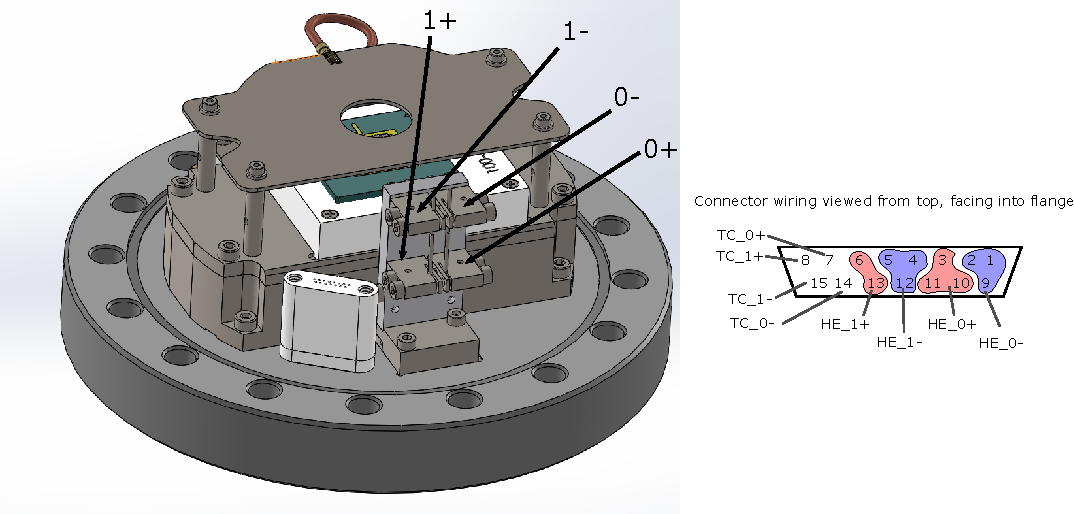
\includegraphics[scale=1]{figures/baseflange_wiring.pdf} 
    \caption{Wiring of in vacuum oven connector}
    \label{fig:baseflange_wiring}
\end{figure}

\section{Temperature readout}
Run the script in \texttt{oven\_test\_scripts/temperature\_readout} to print out temperature measurements in real time. Touch the thermocouples on each tube one after the other to check that the temperature reading changes.

\clearpage
\section{Low power testing}
Measure the current, voltage, and temperature characteristics of the oven at a low/safe power. Run the script in \texttt{oven\_test\_scripts/low\_power\_heating} and enter the channel of oven to be tested. Use the plotter script to make the graph, and the output should look like figure \ref{fig:low_power_heating}.
This measurement determines that everything is connected correctly, the restance of the oven and wiring, and the polarity of the thermocouple connection.

\begin{figure}
    \center
    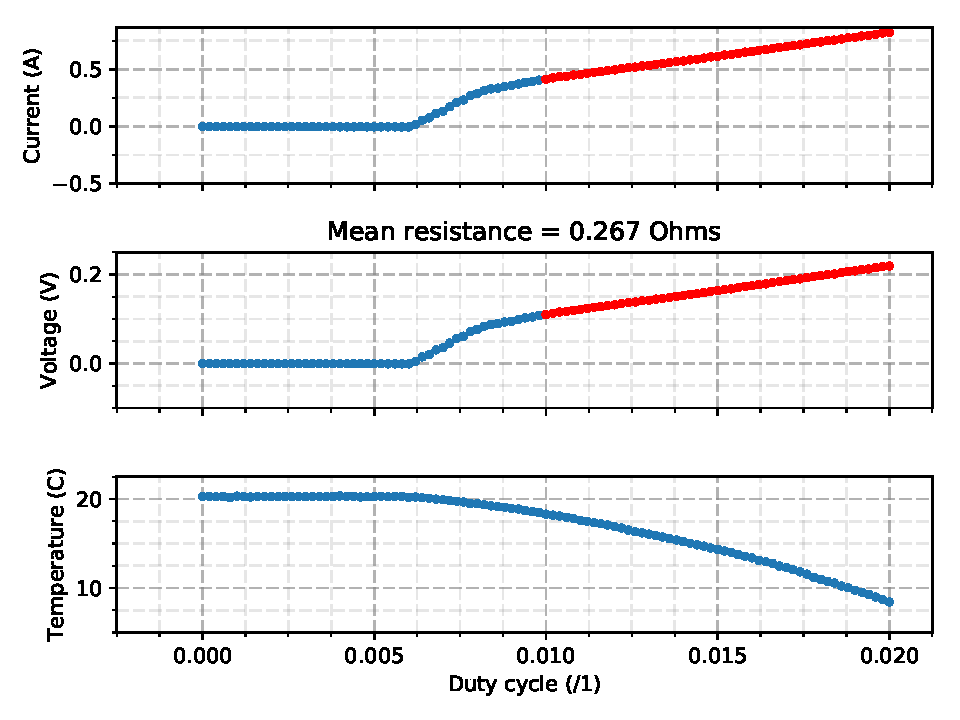
\includegraphics[scale=1]{figures/current_vs_duty_0.pdf} 
    \caption{Example data for low\_power\_heating test. NB if the temperature reading decreases throughout the measurement, this indicates that the sensor polarity is inverted}
    \label{fig:low_power_heating}
\end{figure}

To invert the sensor polarity, run the script \texttt{calibration\_settings/reverse\_tc\_polarity.py} on the channel in question. This will save this configuration in firmware.

\clearpage
\section{Duty impulse response}

This measurement allows us to determine the temperature-current (T-C) cross-coupling of the oven.
This effect occurs when oven current flows through the thermocouple wiring in the vicinity of the spot weld.
Figures \ref{fig:duty_impulse_response_low} and \ref{fig:duty_impulse_response_high} show this measurement when there is a low and high T-C coefficient respectively.

\begin{figure}
    \center
    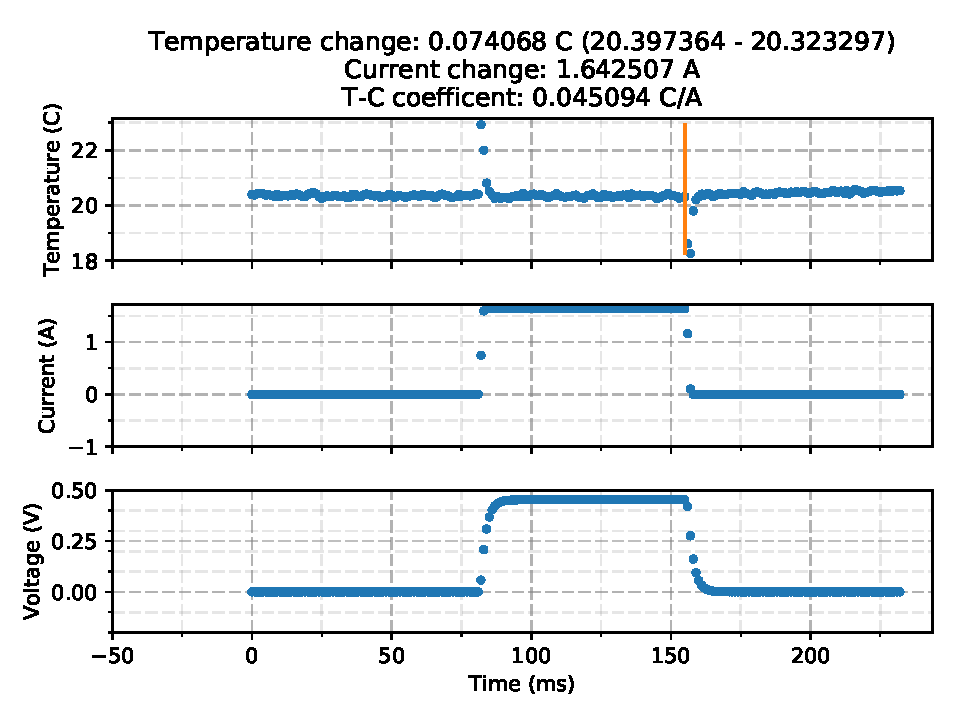
\includegraphics[scale=1]{figures/duty_impulse_response_data_0.pdf} 
    \caption{Example data for "duty impulse response" test where there is a low T-C coefficient.}
    \label{fig:duty_impulse_response_low}
\end{figure}

\begin{figure}
    \center
    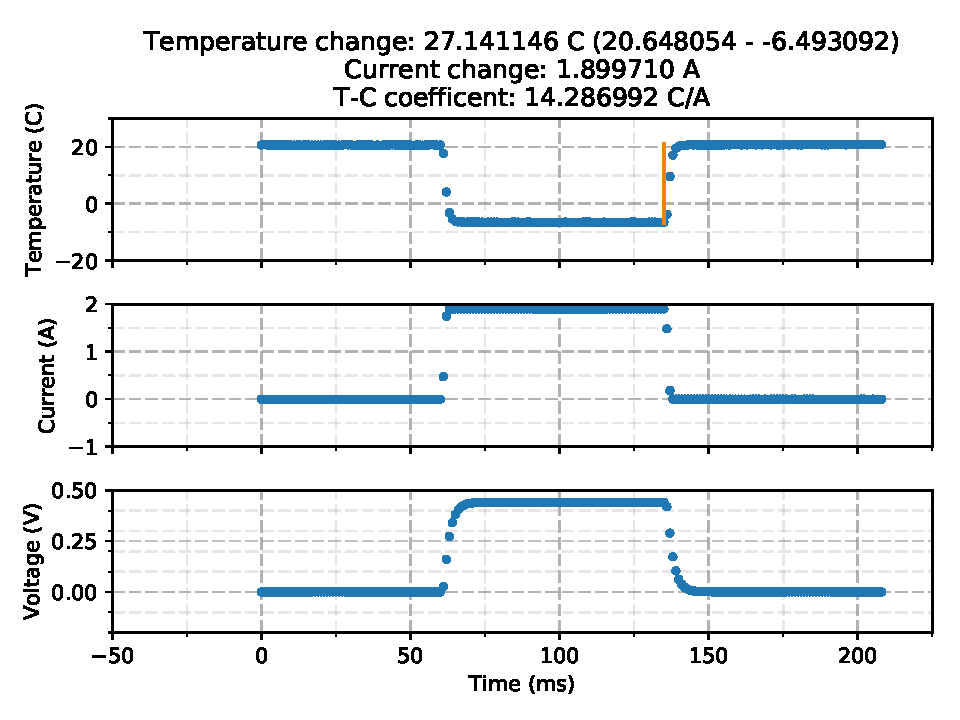
\includegraphics[scale=1]{figures/duty_impulse_response_data_1.pdf} 
    \caption{Example data for "duty impulse response" test where there is a high T-C coefficient.}
    \label{fig:duty_impulse_response_high}
\end{figure}

Once the coupling coefficient is measured, it can be saved in the flash calibration for the microcontroller with the script \texttt{calibration\_settings/set\_tc\_current\_compensation.py}. To confirm that the compensation works, the duty impulse response script can be run again and the measurement should give a much lower coupling value.


\clearpage
\section{Setup current feedback}

Now the current feedback coefficients need to be set for each channel.
The current feedback controller is a PID controller taking a setpoint in Amps and controlling the duty cycle between 0 and 1.

There are four key parameters for this:
\begin{enumerate}
\item P gain,
\item I gain,
\item D gain,
\item Sample decimation\footnote{Sample decimation is the number of samples to skip before applying feedback. The ADC sampling frequency is \SI{1}{kHz}, so a decimation of 0 will lead to \SI{1}{kHz} update rate, whereas decimation of 4 will lead to one sample every 5 ADC samples giving \SI{200}{Hz}. This is useful when the feedback controller needs to act on long timescales compared with the ADC sampling rate}.
\end{enumerate}
These can be adjusted to optimise the performance of the controller, however I have found the following configuration to work in all cases:
0.008, 0.007, 0, 0.

The script \texttt{setup\_current\_feedback/measure\_current\_feedback\_risetime.py} will test the current feedback on the given channel. The feedback controller parameters are set within the script to the values above. The output of this script will result in a plot like the one shown in figure \ref{fig:current_feedback}, which allows us to verify that the feedback controller is working correctly (i.e. no oscillation, reasonable response time).

\begin{figure}
    \center
    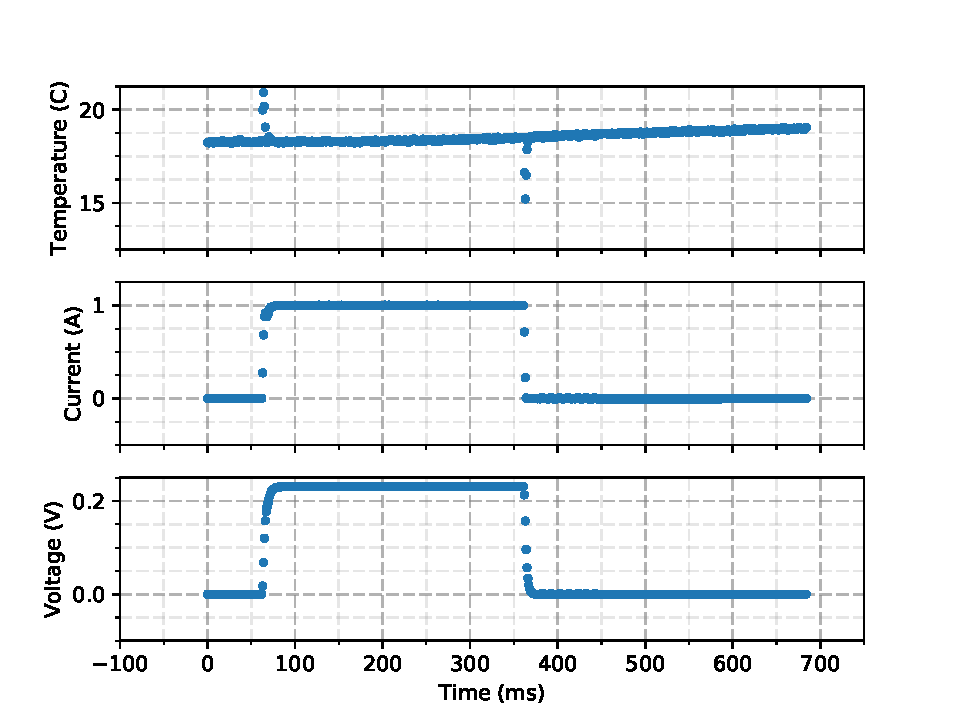
\includegraphics[scale=1]{figures/current_feedback_risetime_data_1.pdf} 
    \caption{Example data for seting up the current controller parameters.}
    \label{fig:current_feedback}
\end{figure}

With the desired current feedback parameters known, program them into the microcontroller with the script in \texttt{calibration\_settings/set\_current\_controller\_settings.py}. This script also asks for the following parameters:
\begin{enumerate}
\item Min/max duty cycle soft limits
\item Maximum setpoint (A)
\item Maximum setpoint slew rate (A/s)
\end{enumerate}


\clearpage
\section{Setup temperature feedback}



\end{document}
